
\documentclass[11pt, a4paper]{report}
\usepackage{graphicx}
\usepackage{fullpage}
\usepackage{url}
\usepackage{listings}
\usepackage{hyperref}
\usepackage{setspace}

\headsep = 25pt

\setlength{\parskip } {0pt}
\begin{document}
\begin{center}

\includegraphics[scale=1.5]{./image/UniLogo}\\[3cm] 

\textbf{\Huge Path Finding Test Report}\\[3cm]

{\LARGE NXT Archeology Robot Test Report }\\[6cm]

\textbf{\large Yunyao Yao }\\[1cm]

\textbf{\large ID: 1203525}\\
\end{center}

\pagebreak
\oddsidemargin -0.5 cm
\evensidemargin -0.5 cm
\textwidth 15 cm
\topmargin -1.2 cm
\textheight 25 cm



\chapter{Test Plan}

\section{Tested Methods}
In these tests, I tested the methods in the PathFinder class including DFS and setPath and the sub-method they call. These class is used for robot's path finding. When a robot starts a auto-navigation, It will call DFS method in this class to search the map. If the robot goes into a dead end and there are still unexplored area, it will call setPath method to find a path from current location to closest unexplored area.As these part of code is not written by me, it would be better to let me to test it rather than the author.\\

\paragraph{}Tested Method Link:

\begin{lstlisting} 
sep2012-13\Code\Final Version\src\Navigation\PathFinder.java
\end{lstlisting} 





\subsection{DFS}
This is a pathFinding method of the robot.It takes a starting point as parameter. It will find a unexplored ( not wall, not no-go zone ) Pixel following this order: North, South, West, East. It store the path it travels by saving a integer into the variable PrevMark of each pixel in the path. For example, "PrevMark=1" means the the previous pixel of current one is at north ( see the table below for more definition ). If robot goes into a dead end which mean no more available moves this method will return. Return value "1" means no more unexplored pixels left in the map, the survey is complete perfectly. Return value "0" means the robot went into a dead end and unfortunately there are still unexplored pixel in the map.

\begin{center}
\begin{tabular}{| l | l | }
\hline
PrevMark		&	Meaning\\ \hline

1 		&	Previous: North\\ \hline
2 		&	Previous: East\\ \hline
3 		&	Previous: South\\ \hline
4		&	Previous: West\\ \hline

\end{tabular}
\end{center}

\subsection{SetPath}
setPath is also a path finding method. However, rather than a single parameter like DFS, it takes two parameters, starting point and destination point. It will return a path from the starting point to destination point as a LinkedList of Pixels. The method will add all pixels on the path in order. Then robot can follow this path to reach the unexplored area.





\section{Test Strategy}
I used JUnit test tools to test the code. For DFS I examine the PrevMark variable of Pixel Objects which marked previous Pixel by direction. For setPath I examine the LinkedList it returns with the LinkedList a build manually.

\section{Pass/Fail Criteria}
\subsection{DFS}
For each Pixel if the value of PrevMark are equal to what I expect in the graph(showed below in each test case).

\subsection{setPath}
The LinkedList this method returns is equal to the one a manually build which contains all the pixels in the expected path.




\chapter{Test Cases} 
I have 5 test cases in total in my test script. For each test case I create a 4 by 4 small map and tested both two methods. The map I created come with walls to block the way of the robot.

\section{Test 1}

\subsection{Map Used In This Test:}
\begin{center}
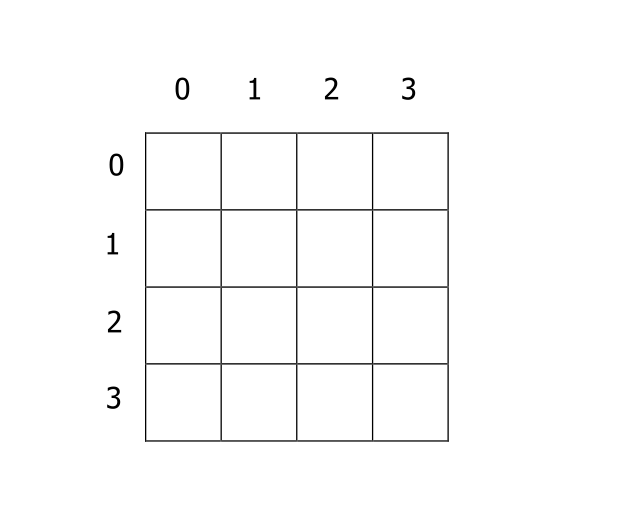
\includegraphics[scale=0.4]{./image/Test1.png}
\end{center}

No wall is set in this test case.\\
\subsection{Reason For Choosing This Case}
This map has no walls, it is designed in order to test that whether the robot can go through the whole map if there is no obstacle.

\subsection{DFS}
Start at (0,0):
\begin{center}
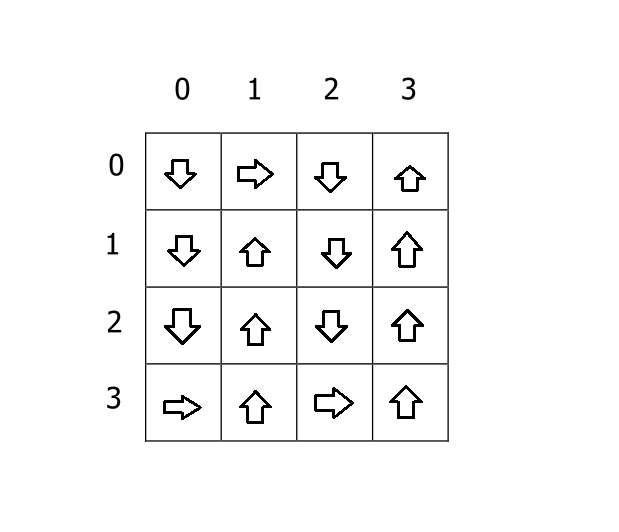
\includegraphics[scale=0.4]{./image/Test1DFS.png}
\end{center}
DFS are expected to search the map like this. So the value of PrevMark is checked by every pixel:\\

\paragraph{}PrevMark Value Diagram:
\begin{center}
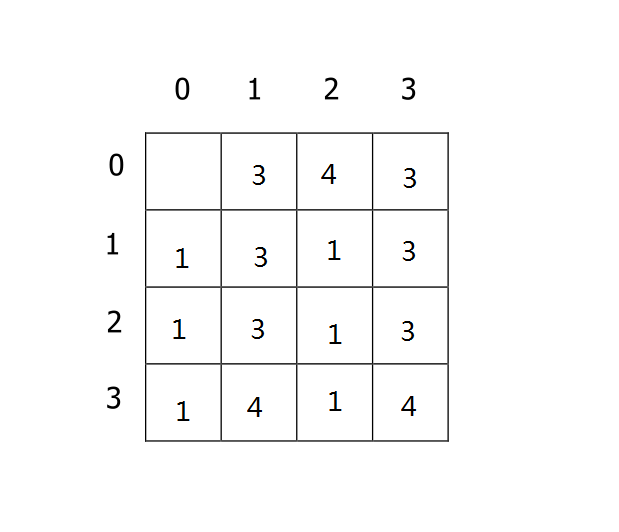
\includegraphics[scale=0.4]{./image/Test1DFSP.png}
\end{center}

\subsection{SetPath}
\paragraph{}Set a Path From (0,0) to (3,3), the expected result is showed below:\\
\begin{center}
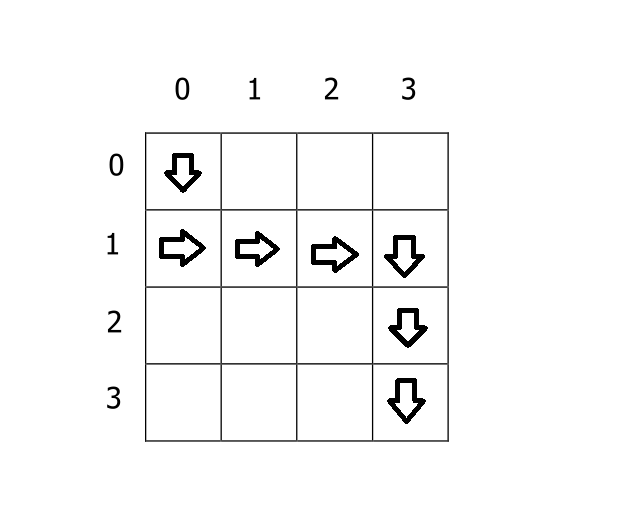
\includegraphics[scale=0.4]{./image/Test1SetPath.png}
\end{center}
\paragraph{}All the pixels on this path is added to a LinkedList, and it will be compared with the return value of SetPath method.



\section{Test 2}

\subsection{Map Used In This Test:}
\begin{center}
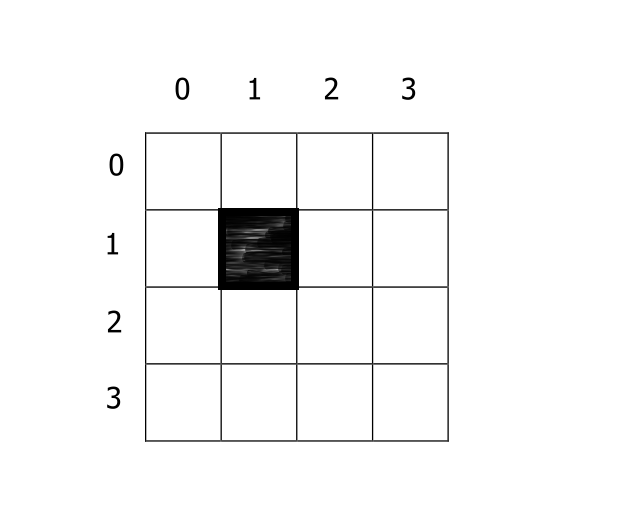
\includegraphics[scale=0.4]{./image/Test2.png}
\end{center}

\noindent (1, 1) is set as wall in this test case.

\subsection{Reason For Choosing This Case}
This map has only one wall. It is designed in order to test that whether it will reached expected location at the end, if robot' path is blocked at the beginning.

\subsection{DFS}
Start at (0,0):
\begin{center}
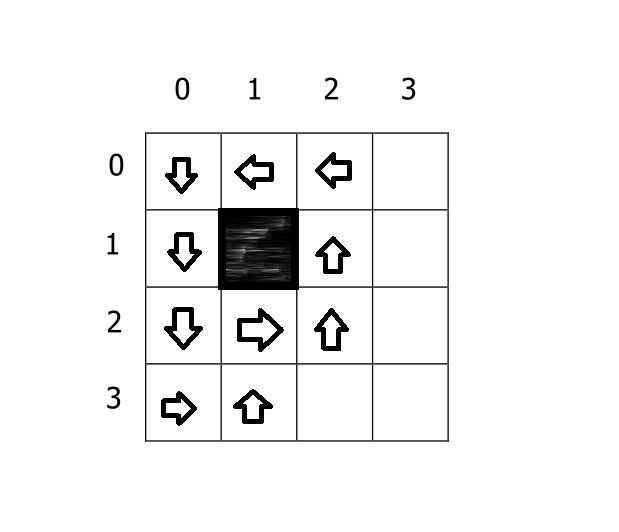
\includegraphics[scale=0.4]{./image/Test2DFS.png}
\end{center}
DFS are expected to search the map like this. So the value of PrevMark is checked by every pixel:\\

\paragraph{}PrevMark Value Diagram:
\begin{center}
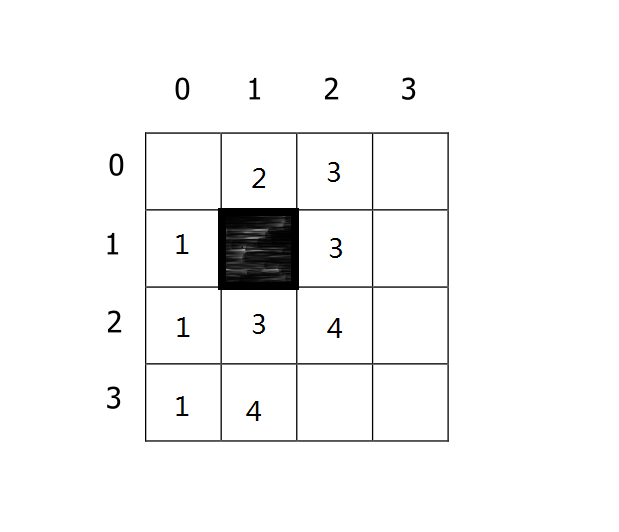
\includegraphics[scale=0.4]{./image/Test2DFSP.png}
\end{center}

\subsection{SetPath}
\paragraph{}Set a Path From (1,0) to (3,3), the expected result is showed below:\\
\begin{center}
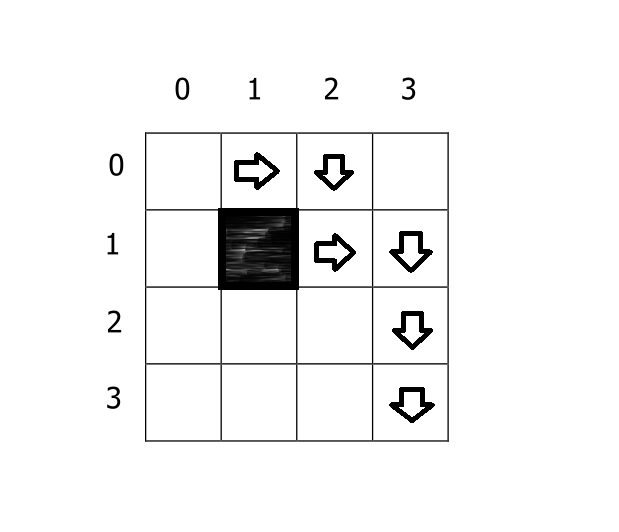
\includegraphics[scale=0.4]{./image/Test2SetPath.png}
\end{center}
\paragraph{}All the pixels on this path is added to a LinkedList, and it will be compared with the return value of SetPath method.



\section{Test 3}

\subsection{Map Used In This Test:}
\begin{center}
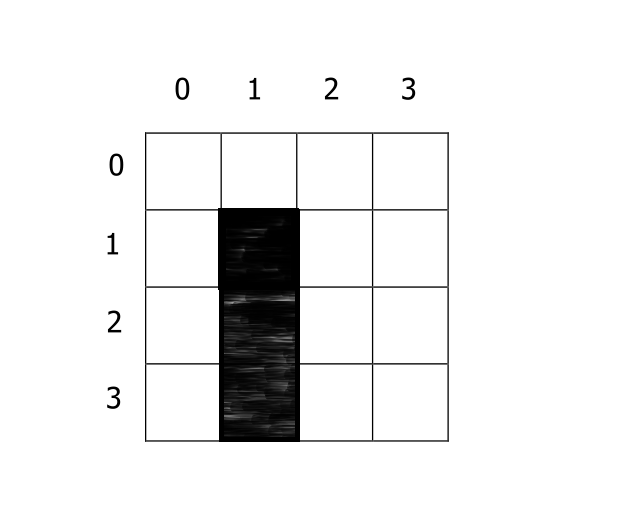
\includegraphics[scale=0.4]{./image/Test3.png}
\end{center}

\noindent (1, 1) is set as wall in this test case.\\
(1, 2) is set as wall in this test case.\\
(1, 3) is set as wall in this test case.\\

\subsection{Reason For Choosing This Case}
This map has a dead-end, and it is designed to test that whether the method can correctly return after the robot go into a dead-end.

\subsection{DFS}
Start at (0,0):
\begin{center}
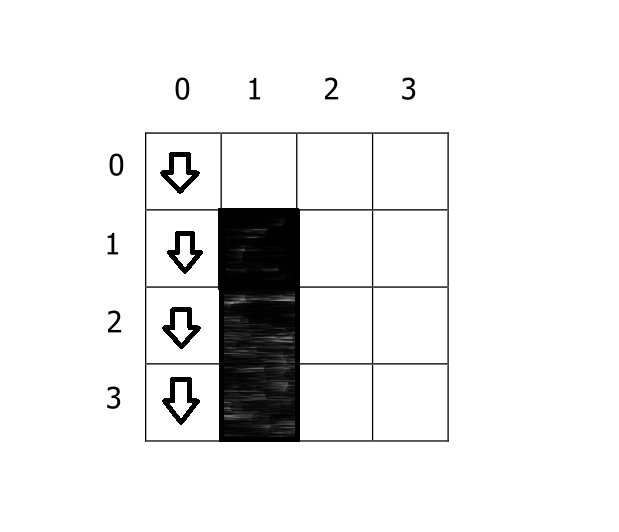
\includegraphics[scale=0.4]{./image/Test3DFS.png}
\end{center}
DFS are expected to search the map like this. So the value of PrevMark is checked by every pixel:\\

\paragraph{}PrevMark Value Diagram:
\begin{center}
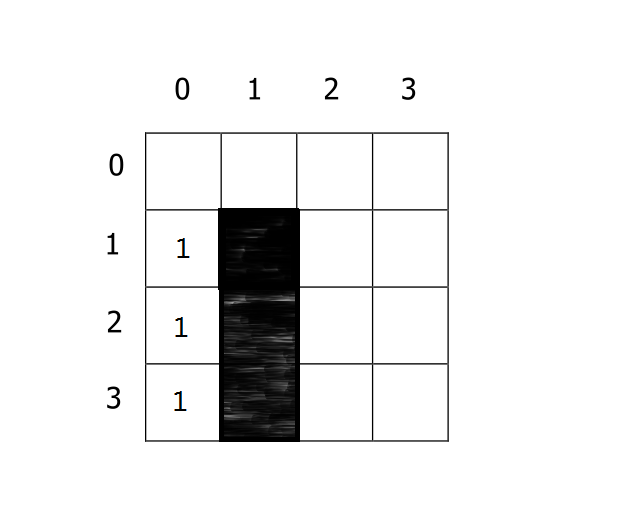
\includegraphics[scale=0.4]{./image/Test3DFSP.png}
\end{center}

\subsection{SetPath}
\paragraph{}Set a Path From (0,3) to (2,3), the expected result is showed below:\\
\begin{center}
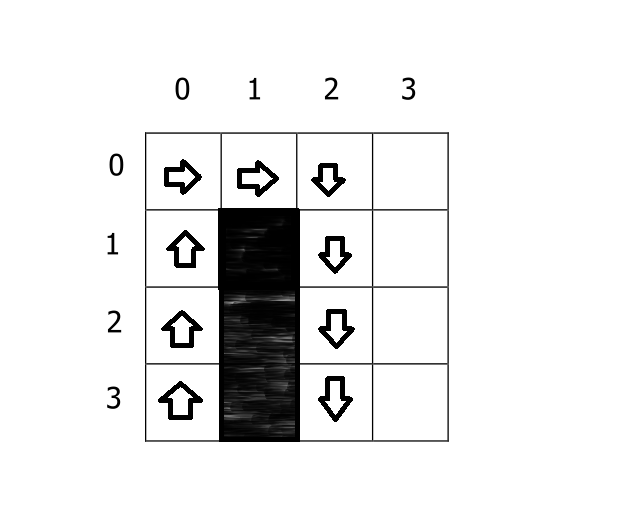
\includegraphics[scale=0.4]{./image/Test3SetPath.png}
\end{center}
\paragraph{}All the pixels on this path is added to a LinkedList, and it will be compared with the return value of SetPath method.



\section{Test 4}

\subsection{Map Used In This Test:}
\begin{center}
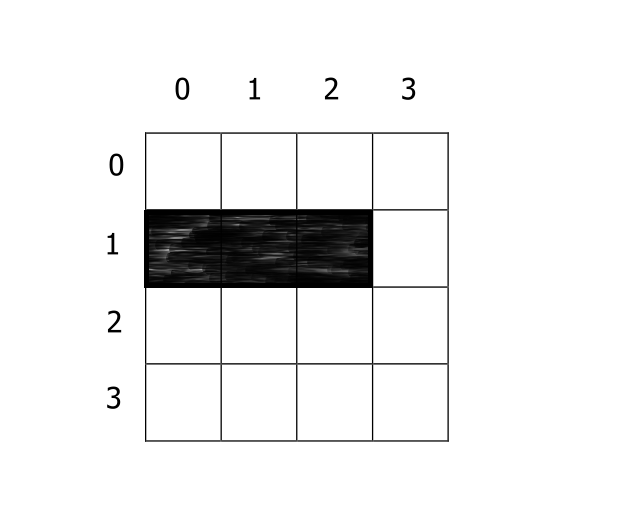
\includegraphics[scale=0.4]{./image/Test4.png}
\end{center}

\noindent (0, 1) is set as wall in this test case.\\
(1, 1) is set as wall in this test case.\\
(2, 1) is set as wall in this test case.\\

\subsection{Reason For Choosing This Case}
This map has walls, but the robot should be able to go through all the pixels in this case, this case is to test that whether it can go through this map.
\subsection{DFS}
Start at (0,0):
\begin{center}
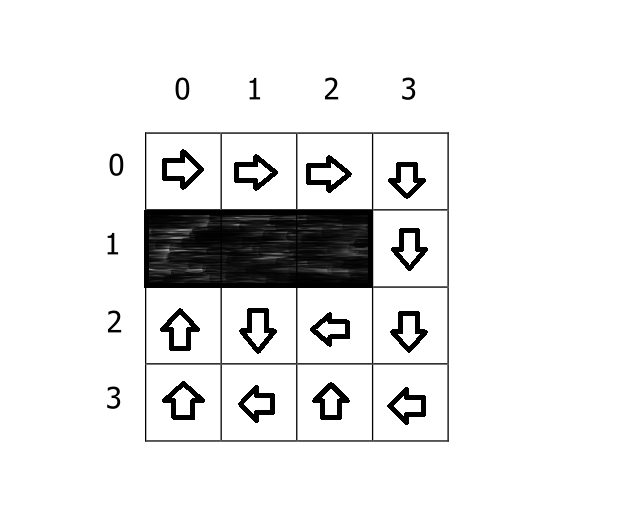
\includegraphics[scale=0.4]{./image/Test4DFS.png}
\end{center}
DFS are expected to search the map like this. So the value of PrevMark is checked by every pixel:\\

\paragraph{}PrevMark Value Diagram:
\begin{center}
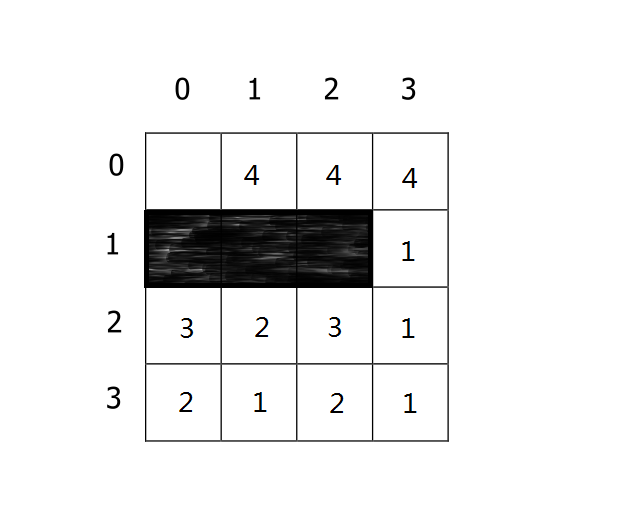
\includegraphics[scale=0.4]{./image/Test4DFSP.png}
\end{center}

\subsection{SetPath}
\paragraph{}Set a Path From (0,2) to (0,0), the expected result is showed below:\\
\begin{center}
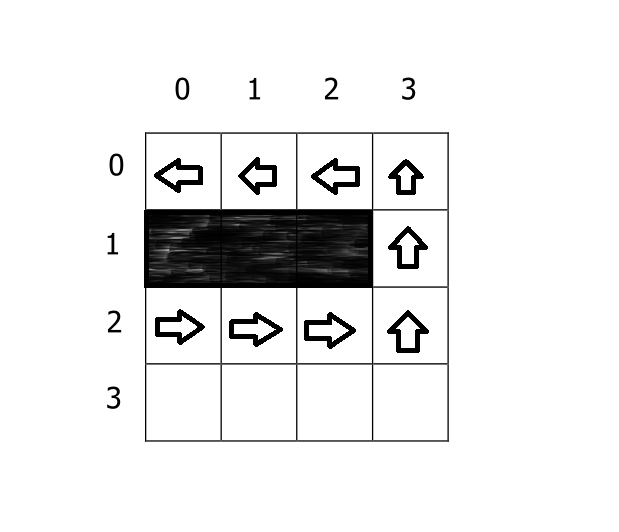
\includegraphics[scale=0.4]{./image/Test4SetPath.png}
\end{center}
\paragraph{}All the pixels on this path is added to a LinkedList, and it will be compared with the return value of SetPath method.


\section{Test 5}

\subsection{Map Used In This Test:}
\begin{center}
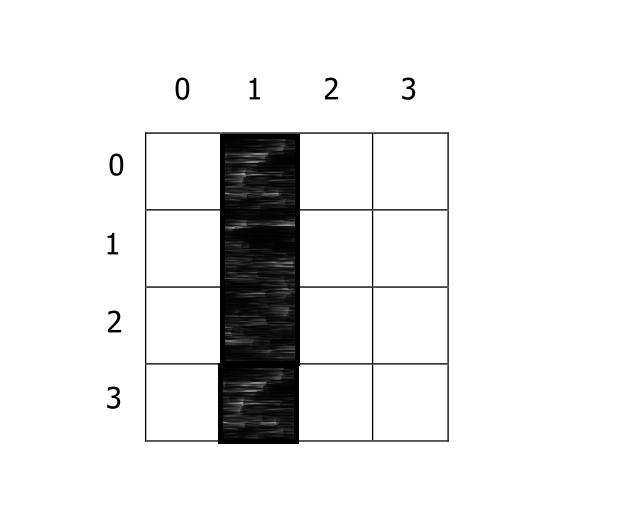
\includegraphics[scale=0.4]{./image/Test5.png}
\end{center}

\noindent (1, 0) is set as wall in this test case.\\
(1, 1) is set as wall in this test case.\\
(1, 2) is set as wall in this test case.\\
(1, 3) is set as wall in this test case.\\

\subsection{Reason For Choosing This Case}
This map is map is separated by walls. This case is designed to test that whether the robot can correctly go through part of the map with DFS and find out that the path is blocked.

\subsection{DFS}
Start at (0,0):
\begin{center}
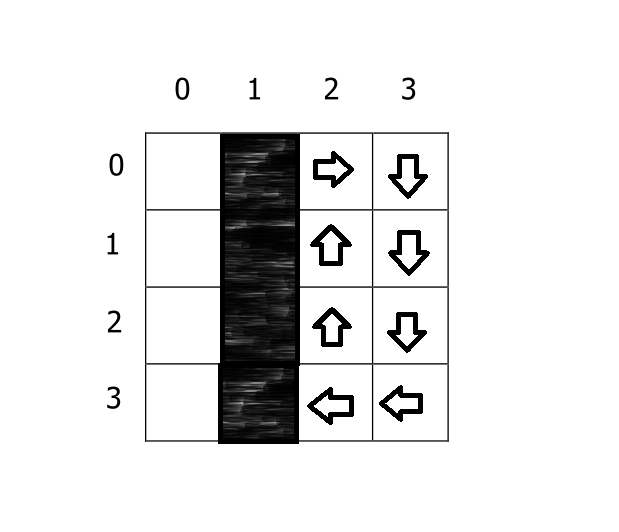
\includegraphics[scale=0.4]{./image/Test5DFS.png}
\end{center}
DFS are expected to search the map like this. So the value of PrevMark is checked by every pixel:\\

\paragraph{}PrevMark Value Diagram:
\begin{center}
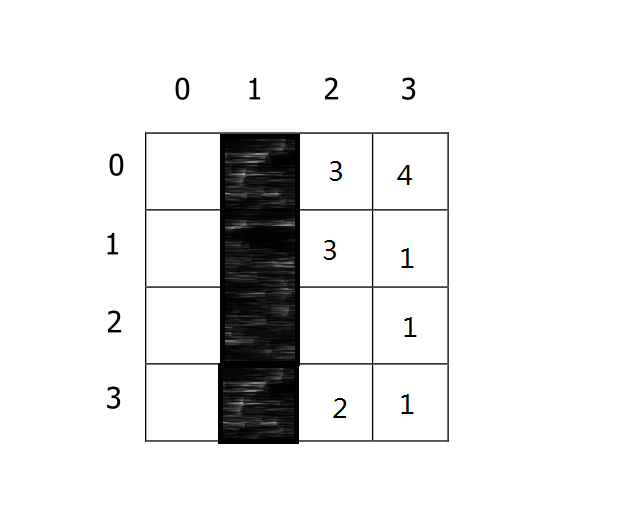
\includegraphics[scale=0.4]{./image/Test5DFSP.png}
\end{center}

\subsection{SetPath}
\paragraph{}Set a Path From (0,2) to (2,2), the expected result is showed below:\\
\begin{center}
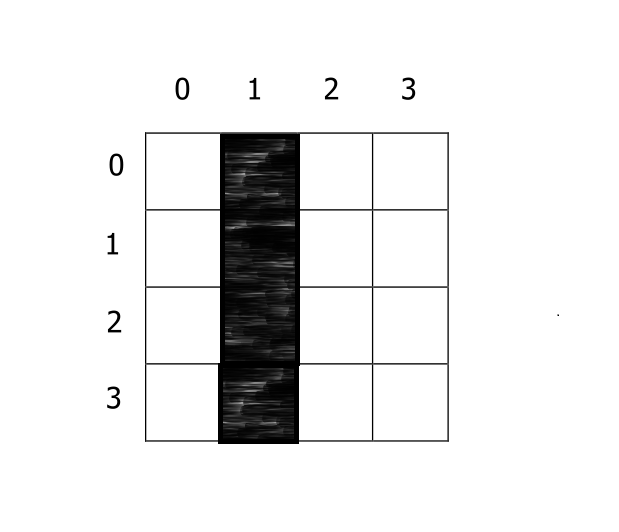
\includegraphics[scale=0.4]{./image/Test5SetPath.png}
\end{center}
\paragraph{}As there is no path from (0,2) to (2,2) the method should return null.


\end{document}